\textbf{Appendice al capitolo III}

Si consideri questa posizione:

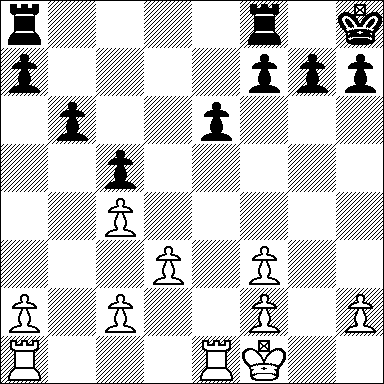
\includegraphics[width=1.40139in,height=1.40139in]{assets/diagrams/image68.png}

\emph{diagramma 68}\\
\emph{muove il Bianco}

Basandosi solo su considerazione generali, senza cioè eseguire calcoli
approfonditi, si domanda chi è preferibile.

Proposi questo esercizio in area \emph{Scacchi-ARS} di Mc link. il BBS
della rivista McMicrocomputer. Ecco che cosa risposero due utenti:

\emph{Paolo Maria Giardini (Petrignano Lago)} : ``A lume di naso direi
che il Nero è messo meglio. A parità di pezzi ha l'arrocco intatto
mentre il Bianco ha due pedoni impedonati ed un buco in g2. Inoltre ha
dei pedoni isolati che lasciano spazio alle manovre dell'avversario. Il
Nero ha invece uno schieramento di pedoni più omogeneo''.

\emph{Gabriele Morra (Roma, all'epoca moderatore dell'area)} : ``... io
preferisco, come Paolo, il Nero. Il motivo risiede soprattutto nella
grande debolezza e isolamento in cui si trovano i pedoni sull'ala di Re
del Bianco. Per quanto riguarda l'ala di Donna, infatti, penso che il
relativo svantaggio dei pedoni doppiati sia ben compensato dalla colonna
\emph{b} libera e dalla posizione relativamente infelice del pedone nero
sempre sulla colonna b. Infatti, anche se questo può essere difeso dal
pedone a7, il Nero può sempre portare una specie di attacco di minoranza
(riferito alle colonne \emph{a} e \emph{b}) con il pedone a2. Come forse
sta un pochino meglio il Bianco, ma dall'altra parte i pedoni bianchi
davanti al Re mi paiono così isolati ed indifesi da essere determinanti
a favore del Nero dicevo, quindi, sull'ala di Donna e al centro la
situazione mi pare pari, anzi in un eventuale ma molto probabile
finale''.

La posizione del diagramma mi è capitata giocando, col Bianco, in una
partita lampo contro un CM senese. Arrivati a questo punto il mio
avversario esclamò: ``Finalmente una posizione dove sto meglio!'' e io
dissi: ``Ma veramente pensavo di stare meglio io!''.

Entrambi avevamo \emph{visto} con qualche mossa d'anticipo questa
posizione ma l'avevamo valutata in modo opposto! Sia Paolo che Gabriele
fanno delle considerazioni valide. Il Bianco ha ben due pedoni doppiati,
un lato di Re sfasciato ecc. ma la domanda che bisogna porsi è: il Nero
può sfruttare queste debolezze?

Un giocatore può avere un buco nella sua posizione, macroscopico quanto
si vuole, ma se l'avversario non ha modo di sfruttarlo quella debolezza
non ha conseguenze. Nella posizione del diagramma, per esempio, i pedoni
bianchi sulla colonna \emph{f} ed \emph{h} sono deboli ma come può il
Nero attaccarli? Certo, se il Pf7 (o h) si trovasse in d7 allora sarebbe
tutto un altro discorso; il Nero potrebbe raddoppiare le Torri sulla
colonna \emph{f (}h) e giocare per vincere ma così non è. Certo, se in
gioco ci fossero ancora dei pezzi minori, e soprattutto la Donna, il
discorso cambierebbe; la debolezza dei pedoni e dell'arrocco si farebbe
sentire parecchio e forse il Nero finirebbe col vincere, ma non è
neanche così.

Passiamo al Nero che, in apparenza, ha una struttura di pedoni perfetta.
Qui Gabriele merita un plauso perché ha capito che sull'ala di Donna,
con le Torri ancora sulla scacchiera, sta meglio il Bianco e soprattutto
ha indicato il piano giusto: l'attacco di minoranza. Infatti, spingendo
il pedone \emph{a} fino in a5 il Nero verrà ad avere inevitabilmente un
pedone debole sul lato di Donna. Avrà deboli i pedoni c5 e il Pa7 in
caso di cambio (b6xa5) oppure quello in b6 se permette al Bianco di
cambiare lui. E, attenzione, questo pedone debole sarà sottoposto a una
forte pressione da parte del Bianco grazie alle colonne semiaperte.
Quindi, il Bianco sta meglio! Se poi riuscirà a vincere o dovrà
accontentarsi della patta questo è solo questione di calcolo. La cosa
sorprendente è che tutto il software scacchistico cui ho sottoposto la
posizione è concorde nel preferire il Nero, e sono addirittura i
programmi di maggior prestigio quelli che valutano peggio questa
posizione! Si pensi, per esempio, che lo Psion chess valuta in leggero
il vantaggio del Nero mentre l'Mchess 1.71 (uno dei migliori sul
mercato, valuta il Nero in vantaggio di oltre 1 punto e mezzo (cioè un
pedone e mezzo!). Naturalmente non ho avuto difficoltà a battere e il
mio avversario e gli altri programmi cui ho sottoposto la posizione.

Ecco come è continuata la partita con l'Mchess:

\textbf{1.a4 ¦fc8 2.¦fbl ¦c7 3.¦b5 ¢g8 4.a5 ¦b8} il candidato maestro
senese preferì 2... bxa5 ma la mossa del calcolatore è migliore.

\textbf{5.¦ab1 T¤b7 6.d4 ¤xd4 7.c5 ¦bc8 8.a6 ¦bb8 9.¤xb6 ¦xb6 10.¦xb6
axb6 11.a7 ¦a8 12.¦xb6} e vince.

Si rimettano i pezzi nella posizione del diagramma. Se, al posto di 3...
¢g8, il Nero avesse giocato 3... g6 alla 12\textsuperscript{a} mossa si
sarebbe assistito a una corsa per il controllo di b7:

\textbf{12.¦a1 ¢g7 13.¢e2 ¢f8 14.¢d3 ¢e7 15.¢c4 ¢d6 16.¢b5 ¢c7 17.¢a6!}
e vince perché la Torre è libera di muoversi e il Nero non ha modo di
impedire uno scacco sulla colonna ``c'' (¦a4 ¦c4+) e la successiva
entrata in b7 del Re Bianco.

Forse i programmatori si sono dimenticati di insegnare al software che
l'attacco di minoranza equivale a un pedone isolato virtuale~\ldots{} o
forse no. Forse l'Mchess ha valutato il suo futuro pedone isolato ma
continuava a darsi in vantaggio perché il Bianco ne ha più di uno. Forse
invece non considera abbastanza il vantaggio della colonna semiaperta o
non tiene conto del fatto che sulla scacchiera ci sono solo le Torri.

Insomma, appare ovvio, come i programmi siano ancora carenti dal punto
di vista strategico.

Quando i programmatori saranno riusciti a formalizzare in modo fine la
strategia del gioco degli scacchi, bè a quel punto, data la loro enorme
capacità di calcolo, ci batteranno senza problemi (non sarà comunque la
fine degli scacchi che sono, innanzitutto, competizione intellettiva, di
volontà, psicologica ecc., tra due esseri umani). Ma non è compito
facile.

Si consideri questa semplice posizione:

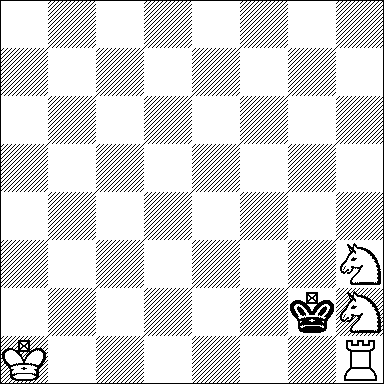
\includegraphics[width=1.40139in,height=1.40139in]{assets/diagrams/image69.png}

\emph{diagramma 69}

Tratto al Nero.

È evidente che basta prendere in h1 per pareggiare. Tutto il software
che c'è in giro gioca invece l... ¢xh3\footnote{Nota del 30.1.1996:
  rispetto a quando scrissi queste note il problema è stato risolto e
  oggi tutto il software prende la Torre. La validità dell'esempio
  comunque rimane a testimonianza delle difficoltà cui vanno incontro i
  programmatori di scacchi.} perché \emph{vede} che dopo 2. ¤f1 ¢g2
cattura un secondo pezzo (e due Cavalli, gli è stato giustamente
insegnato, valgono più di una Torre); purtroppo non gli è stato detto
che la Torre da sola riesce a dare matto e i due Cavalli no, e così il
poveretto perde la partita. Naturalmente è facile dargli questa
informazione ma non è banale arrivare a formalizzare tutto il gioco
degli scacchi.

Gli uomini agiscono in modo diverso. Leggono, per esempio, di vari
elementi strategici e basta loro usarli anche poche volte per riuscire a
valutare in modo sorprendentemente preciso l'importanza di uno di essi
in relazione agli altri, data una qualsiasi posizione. Come il cervello
umano possa essere tanto preciso affidandosi a valutazioni generiche,
Dio solo lo sa. Al calcolatore va spiegato tutto in modo certosino ed è
ovvio che, innanzitutto, gli uomini debbano spiegare i meccanismi di
valutazione a se stessi. L'altro metodo per batterci, data la difficoltà
a formalizzare in modo fine gli scacchi, è aumentare a dismisura le
capacità di calcolo (forza bruta). Se ci fosse un calcolatore così
potente da riuscire a calcolare tutto il finale del diagramma
scoprirebbe da solo che la Torre vince e i due Cavalli no, e agirebbe di
conseguenza. Purtroppo sembra questa scorciatoia la strada scelta dai
programmatori; e dico purtroppo perché costruire un supercalcolatore che
spara mosse su mosse come un pazzo da manicomio servirà poco e agli
scacchisti e agli studiosi di Intelligenza Artificiale.
